% !TeX root = skripta-konstitutivni-vztahy-materialu.tex
% !TeX lastmodified = 2019-12-06

\subsection{Model plastického tečení Ramberg-Osgood}\label{sec:ramberg-osgood}
Tento model\footnote{Ramberg, W., Osgood, W. R. "Description of stress-strain curves by three parameters", Technical Note No. 902, National Advisory Committee For Aeronautics, Washington DC, 1943} vyjadřuje explicitně logaritmické přetvoření jako funkci skutečného napětí nezávislou na čase; je vhodný pro materiály bez výrazné meze kluzu.

Je popsán rovnicemi
\begin{equation}
	\varepsilon = \frac{\sigma}{E} + K \left( \frac{\sigma}{E} \right)^n,
\end{equation}
nebo
\begin{equation}
	\varepsilon = \frac{\sigma}{E} + 0.002 \left( \frac{\sigma}{\sigma_y} \right)^n,
\end{equation}
kde
\begin{description}
	\item[$\varepsilon$] je (celkové) přetvoření,
	\item[$E$] je Youngův modul,
	\item[$\sigma_y$] je mez kluzu ($R_{p0.2}$),
	\item[$n$] je parametr modelu,
	\item[$K$] je parametr modelu.
\end{description}

Model popisuje celou křivku elastické deformace i~zpevnění jedinou obecně nelineární mocninnou funkcí, protože pracuje pouze s~celkovým přetvořením.
Pro víceosou napjatost se použije jako skalární hodnota $\sigma$ redukované von Misesovo napětí a~výsledné $\varepsilon$ je redukované přetvoření.

\subsubsection{Použitelnost modelu plastického tečení}
Plastické tečení často významně závisí na rychlosti zatěžování, tedy je de facto viskoplastické.
Mezní plocha plasticity pak závisí na rychlosti zatěžování.

Plastické modely, které nezohledňují rychlost zatěžování, lze použít:
\begin{itemize}
	\item při velmi (nekonečně) malých rychlostech zatěžování -- vnitřní křivka na obrázku \ref{fig:mezni_plocha_plasticity} (nedojde k porušení termodynamické rovnováhy),
	\item při velmi vysokých rychlostech zatěžování -- vnější křivka na obrázku \ref{fig:mezni_plocha_plasticity} (rázové děje),
	\item při absolutní teplotě do $\frac{1}{4}$ teploty tavení kovu, kdy je rozdíl mezi oběmi křivkami zanedbatelný.
\end{itemize}

\begin{figure}[H]
	\centering
	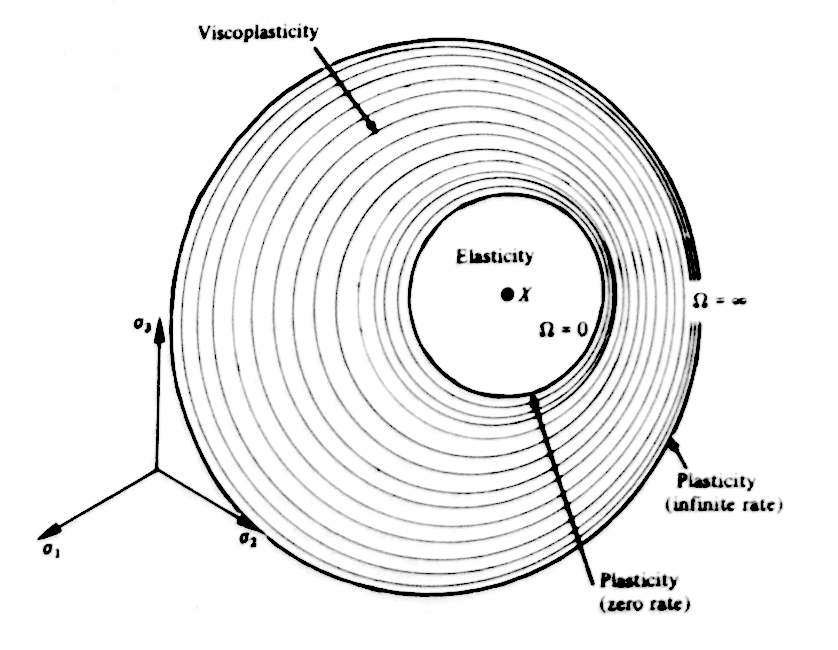
\includegraphics[width=0.8\textwidth]{zavislost-mezni-plochy-plasticity}
	\caption{Závislost mezní plochy plasticity na rychlosti zatěžování}
	\label{fig:mezni_plocha_plasticity}
\end{figure}
